\apendice{Especificación de diseño}

\section{Introducción}

En esta sección se describirá el diseño de la aplicación en sus diferentes componentes:
\begin{itemize}
    \item Arquitectura: patrones de diseño, uso de ASP.NET Core y Modelo Vista-Controlador.
    \item Base de datos: diseño de tablas con \emph{code-first} y migraciones desde Visual Studio.
    \item Estructura: funcionalidad y diseño de las vistas de la aplicación.
\end{itemize}

\section{Diseño arquitectónico (patrones, lenguaje, dependencias...)}

La aplicación utiliza como \emph{framework} principal .NET (versión 6.0), con el marco de trabajo ASP Core, que es un multiplataforma dedicado a proyectos de entorno y desarrollo web. Al ser en Core, el lenguaje que se utiliza es C\#, que es el encargado de la estructura principal del programa (lado del controlador), aunque también se hará uso de JavaScript y html (lado de las vistas).

El patrón arquitectónico que se va a utilizar es el Modelo Vista-Controlador, que separa, por un lado, la estructura y funcionalidad principal del programa, y por otro, las vistas web y su funcionalidad. 

\begin{figure}
    \centering
    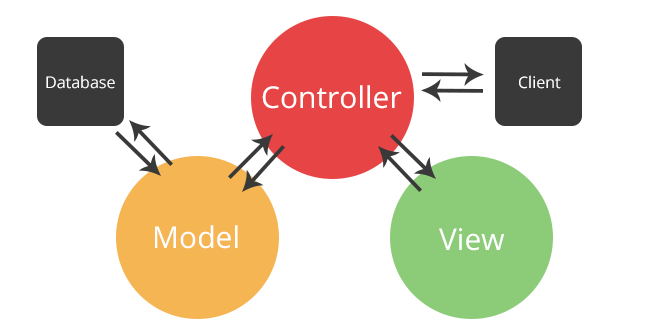
\includegraphics[width=\linewidth]{MVC}
    \caption{Modelo Vista-Controlador}
    
\end{figure}

Esta arquitectura permite estructurar la aplicación en tres capas y relacionarlas entre ellas:
\begin{itemize}
 \item \textbf{Modelo}: estructura interna de los datos (clases y modelos de las tablas de la base de datos).
 \item \textbf{Controlador}: clase que se encarga de obtener datos del modelo o de enviar estos al mismo. Es el puente entre la vista y los modelos.
 \item \textbf{Vista}: visualiza los datos del modelo que son enviados por el controlador, es la forma de interacción entre el cliente y el servidor, y se comunica de nuevo con el controlador para enviar peticiones o datos de vuelta al modelo. 
 \end{itemize}
 
El lado del modelo y el de las vistas se unen a través de llamadas por parte de ambos (redirecciones a las vistas, creación de modelos y acciones del controlador en el lado del controlador, y peticiones \emph{GET} y \emph{POST} desde el lado de las vistas).

La aplicación de este patrón funciona de la siguiente forma:
\begin{itemize}
    \item 1º. El controlador es el elemento principal, hace las redirecciones de las vistas y crea los modelos (objetos con elementos de la base de datos que se pasarán a la vistas para rellenar campos).
    \item 2º. El modelo es el elemento intermedio, se pasa a la vista para cargar los datos principales. Las vistas son la cara visible de la aplicación, de forma que el usuario puede editar o añadir datos en estas, y reenviarlos de nuevo al controlador.
    \item 3º. A través de peticiones \emph{GET} y \emph{POST} en las vistas, ya sea con formularios o con \emph{Ajax} (librería de JavaScript para hacer llamadas al controlador), la parte de la vista se comunica con el controlador y envía los datos.
\end{itemize}

\section{Diseño de Base de Datos}
Al trabajar con Core, a la hora de añadir/quitar/modificar tablas se realizará todo en code first. Code first es una forma de definir el modelo en dirección clase -> tabla, de forma que se define la estructura de la base de datos creando primero las clases del modelo o de las entidades que se utilizan en la aplicación. 

Los elementos necesarios para crear la estructura de la base de datos son los siguientes:
\begin{itemize}
    \item Clases/modelos de las tablas que se quieren añadir.
    \item Configuración de la cadena de conexión a la base de datos desde el archivo de configuración de la aplicación (appconfig.json, es un archivo que especifica, entre otros elementos, la cadena de conexión a la BD).
    \item Contexto de la aplicación (es un objeto del tipo Database Context que hace de nexo o puente entre el proyecto y la base de datos). El contexto se llena con las instancias de las clases que vamos a crear, y estas se migran a la base de datos a través de este.
    \item Consola del administrador de paquetes para migrar (añadir todos los nuevos cambios a la base de datos) y actualizar las tablas de la base de datos.
\end{itemize}

Las migraciones en Core son la forma en la que se actualiza la base de datos con los nuevos cambios de clases/atributos. El proyecto tiene un \emph{Snapshot}, que es un fichero que guarda la estructura de la base de datos en su última actualización. Si cambiamos o añadimos una clase o una columna, la migración lo compara con la snapshot para saber qué se debe cambiar en la base de datos.

El orden que se sigue para crear o modificar la estructura de la base de datos es:
\begin{itemize}
    \item 1º. Creación de la clase del modelo/tabla que se quiere añadir.
    \item 2º. Instancia de esta clase en el contexto de la aplicación.
    \item 3º. Con la consola del instalador de paquetes, añadir la migración.
    \item 4º. Después de la migración, actualizar la base de datos.
\end{itemize}

\section{Tablas/Modelos de la base de datos}
A continuación se muestran las tablas de la base de datos, con la notación DBM (DataBase Model):

\begin{table}[H]
    \centering
	\begin{tabularx}{\linewidth}{ p{0.25\columnwidth} p{0.61\columnwidth} }
		\textbf{DBM-01}    & \textbf{AptitudCV}\\
		\toprule
		\text{Descripción} & Tabla para almacenar las entradas de Aptitud de los CV's \\		
		\toprule
        \textbf{Campo}          & \textbf{Tipo}\\
        \text{IdAptitudCV}      & int (PK) \\	
        \text{Descripcion}      & nvarchar(max) null \\	
        \text{IdCurriculum}     & int (FK - Curriculum) null\\	
		\bottomrule
	\end{tabularx}
	\caption{DBM-01 AptitudCV}
\end{table}

\begin{table}[H]
    \centering
	\begin{tabularx}{\linewidth}{ p{0.25\columnwidth} p{0.61\columnwidth} }
		\textbf{DBM-02}    & \textbf{Curriculum}\\
		\toprule
		\text{Descripción} & Tabla para almacenar los currículums \\		
		\toprule
        \textbf{Campo}          & \textbf{Tipo}\\
        \text{IdCurriculum}     & int (PK) \\	
        \text{IdUsuario}        & int not null \\	
        \text{FechaCurriculum}  & datetime null \\	
		\bottomrule
	\end{tabularx}
	\caption{DBM-02 Curriculum}
\end{table}

\begin{table}[H]
    \centering
	\begin{tabularx}{\linewidth}{ p{0.25\columnwidth} p{0.6\columnwidth} }
		\textbf{DBM-03}    & \textbf{Departamento}\\
		\toprule
		\text{Descripción} & Tabla maestra de departamentos \\		
		\toprule
        \textbf{Campo}          & \textbf{Tipo}\\
        \text{IdDepartamento}   & int (PK) \\	
        \text{Descripcion}      & nvarchar(50) not null \\	
        \text{Codigo}           & nvarchar(max) null \\	
		\bottomrule
	\end{tabularx}
	\caption{DBM-03 Departamento}
\end{table}

\begin{table}[H]
    \centering
	\begin{tabularx}{\linewidth}{ p{0.25\columnwidth} p{0.60\columnwidth} }
		\textbf{DBM-04}    & \textbf{Entrada}\\
		\toprule
		\text{Descripción} & Tabla para guardar las publicaciones de los usuarios \\		
		\toprule
        \textbf{Campo}          & \textbf{Tipo}\\
        \text{IdEntrada}        & int (PK) \\	
        \text{IdUsuario}        & int (FK - Usuario) not null \\	
        \text{IdProyecto}       & int (FK - Proyecto) nulll \\	
        \text{Lenguaje}         & nvarchar(10) null \\
        \text{TituloIssue}      & nvarchar(50) null \\
        \text{Descripcion}      & nvarchar(150) not null \\
        \text{Editada}          & bit not null \\
        \text{Resuelta}         & bit not null \\
        \text{NumRespuestas}    & int null \\
		\bottomrule
	\end{tabularx}
	\caption{DBM-04 Entrada}
\end{table}

\begin{table}[H]
    \centering
	\begin{tabularx}{\linewidth}{ p{0.25\columnwidth} p{0.61\columnwidth} }
		\textbf{DBM-05}    & \textbf{EntradaCV}\\
		\toprule
		\text{Descripción} & Tabla que guarda la experiencia laboral 
                               de los usuarios de los CV's \\		
		\toprule
        \textbf{Campo}          & \textbf{Tipo}\\
        \text{IdEntradaCV}      & int (PK) \\	
        \text{IdUsuario}        & int (FK - Usuario) null\\	
        \text{IdCurriculum}     & int (FK - Curriculum) null\\	
        \text{Observaciones}    & nvarchar(max) not null \\	
        \text{PuestoTrabajo}    & nvarchar(50) null\\	
        \text{EmpresaAsociada}  & nvarchar(50) null \\	
        \text{Ubicacion}        & nvarchar(max) null \\	
        \text{FechaDesde}       & datetime not null \\	
        \text{FechaHasta}       & datetime not null \\	
		\bottomrule
	\end{tabularx}
	\caption{DBM-05 EntradaCV}
\end{table}

\begin{table}[H]
    \centering
	\begin{tabularx}{\linewidth}{ p{0.25\columnwidth} p{0.61\columnwidth} }
		\textbf{DBM-06}    & \textbf{FormacionCV}\\
		\toprule
		\text{Descripción} & Tabla que guarda la formacion académica 
                               de los usuarios de los CV's \\		
		\toprule
        \textbf{Campo}          & \textbf{Tipo}\\
        \text{IdFormacionCV}    & int (PK) \\	
        \text{IdUsuario}        & int (FK - Usuario) null\\	
        \text{IdCurriculum}     & int (FK - Curriculum) null\\	
        \text{IdTipoFormacion}  & int (FK - TipoFormacion) null\\	
        \text{Grado}            & nvarchar(max) not null \\	
        \text{Descripcion}      & nvarchar(max) null\\	
        \text{Ubicacion}        & nvarchar(max) null \\	
        \text{FechaDesde}       & datetime null \\	
        \text{FechaHasta}       & datetime null \\	
		\bottomrule
	\end{tabularx}
	\caption{DBM-06 FormacionCV}
\end{table}

\begin{table}[H]
    \centering
	\begin{tabularx}{\linewidth}{ p{0.25\columnwidth} p{0.61\columnwidth} }
		\textbf{DBM-07}    & \textbf{EventosUsuario}\\
		\toprule
		\text{Descripción} & Tabla que guarda los eventos programados de los usuarios \\		
		\toprule
        \textbf{Campo}          & \textbf{Tipo}\\
        \text{IdEventoUsuario}  & int (PK) \\	
        \text{IdUsuario}        & int (FK - Usuario) null\\	
        \text{Descripción}      & nvarchar(50) not null \\		
		\bottomrule
	\end{tabularx}
	\caption{DBM-07 EventosUsuario}
\end{table}

\begin{table}[H]
    \centering
	\begin{tabularx}{\linewidth}{ p{0.25\columnwidth} p{0.61\columnwidth} }
		\textbf{DBM-08}    & \textbf{FotoUsuarioCV}\\
		\toprule
		\text{Descripción} & Tabla que guarda la foto de usuario de un currículum
                               específico de un usuario\\		
		\toprule
        \textbf{Campo}          & \textbf{Tipo}\\
        \text{IdFotoUsuarioCV}  & int (PK) \\	
        \text{IdUsuario}        & int (FK - Usuario) null\\	
        \text{IdCurriculum}     & int (FK - Curriculum) null\\	
        \text{Ruta}             & nvarchar(max) null \\	
        \text{Guid}             & nvarchar(36) null\\	
        \text{Ext}              & nvarchar(max) null \\	
		\bottomrule
	\end{tabularx}
	\caption{DBM-08 FotoUsuarioCV}
\end{table}

\begin{table}[H]
    \centering
	\begin{tabularx}{\linewidth}{ p{0.25\columnwidth} p{0.61\columnwidth} }
		\textbf{DBM-09}    & \textbf{Grupo}\\
		\toprule
		\text{Descripción} & Tabla maestra para los grupos\\		
		\toprule
        \textbf{Campo}          & \textbf{Tipo}\\
        \text{IdGrupo}          & int (PK) \\	
        \text{Descripcion}      & nvarchar(50) null \\	
		\bottomrule
	\end{tabularx}
	\caption{DBM-09 Grupo}
\end{table}

\begin{table}[H]
    \centering
	\begin{tabularx}{\linewidth}{ p{0.25\columnwidth} p{0.61\columnwidth} }
		\textbf{DBM-10}    & \textbf{Idioma}\\
		\toprule
		\text{Descripción} & Tabla maestra para los idiomas \\		
		\toprule
        \textbf{Campo}          & \textbf{Tipo}\\
        \text{IdIdioma}         & int (PK) \\	
        \text{Descripcion}      & nvarchar(50) not null \\	
        \text{Codigo}           & nvarchar(5) not null \\	
		\bottomrule
	\end{tabularx}
	\caption{DBM-10 Idioma}
\end{table}

\begin{table}[H]
    \centering
	\begin{tabularx}{\linewidth}{ p{0.25\columnwidth} p{0.61\columnwidth} }
		\textbf{DBM-11}    & \textbf{IdiomaCV}\\
		\toprule
		\text{Descripción} & Tabla que guarda las entradas de los idiomas de un usuario
                               de un currículum específico\\		
		\toprule
        \textbf{Campo}          & \textbf{Tipo}\\
        \text{IdIdiomaCV}       & int (PK) \\
        \text{IdIdioma}         & int (FK - Idioma) null \\
        \text{IdNivelIdioma}    & int (FK - NivelIdioma) null \\
        \text{IdCurriculum}     & int (FK - Curriculum) null \\        
        \text{Descripcion}      & nvarchar(max) not null \\	
        \text{Centro}           & nvarchar(50) not null \\	
        \text{FechaDesde}       & datetime null \\	
        \text{FechaHasta}       & datetime null \\	        
		\bottomrule
	\end{tabularx}
	\caption{DBM-11 IdiomaCV}
\end{table}

\begin{table}[H]
    \centering
	\begin{tabularx}{\linewidth}{ p{0.25\columnwidth} p{0.61\columnwidth} }
		\textbf{DBM-12}    & \textbf{LogroCV}\\
		\toprule
		\text{Descripción} & Tabla para almacenar las entradas de Logro de los CV's \\		
		\toprule
        \textbf{Campo}          & \textbf{Tipo}\\
        \text{IdLogroCV}        & int (PK) \\	
        \text{Descripcion}      & nvarchar(max) null \\	
        \text{IdCurriculum}     & int (FK - Curriculum) null\\	
		\bottomrule
	\end{tabularx}
	\caption{DBM-12 LogroCV}
\end{table}

\begin{table}[H]
    \centering
	\begin{tabularx}{\linewidth}{ p{0.25\columnwidth} p{0.61\columnwidth} }
		\textbf{DBM-13}    & \textbf{NivelIdioma}\\
		\toprule
		\text{Descripción} & Tabla maestra con los niveles de los idiomas \\		
		\toprule
        \textbf{Campo}          & \textbf{Tipo}\\
        \text{IdNivelIdioma}    & int (PK) \\	
        \text{Descripcion}      & nvarchar(50) not null \\	
		\bottomrule
	\end{tabularx}
	\caption{DBM-13 NivelIdioma}
\end{table}

\begin{table}[H]
    \centering
	\begin{tabularx}{\linewidth}{ p{0.25\columnwidth} p{0.61\columnwidth} }
		\textbf{DBM-14}    & \textbf{NotasUsuario}\\
		\toprule
		\text{Descripción} & Tabla para almacenar las notas de usuario \\		
		\toprule
        \textbf{Campo}          & \textbf{Tipo}\\
        \text{IdNotaUsuario}    & int (PK) \\	
        \text{IdUsuario}        & int (FK - Usuario) not null \\	
        \text{Descripcion}      & nvarchar(100) null\\	
        \text{Titulo}      & nvarchar(50) not null\\	
		\bottomrule
	\end{tabularx}
	\caption{DBM-14 NotasUsuario}
\end{table}

\begin{table}[H]
    \centering
	\begin{tabularx}{\linewidth}{ p{0.25\columnwidth} p{0.61\columnwidth} }
		\textbf{DBM-15}    & \textbf{Notificacion}\\
		\toprule
		\text{Descripción} & Tabla para las notificaciones de los usuarios por eventos
                               o respuestas\\		
		\toprule
        \textbf{Campo}              & \textbf{Tipo}\\
        \text{IdNotificacion}       & int (PK) \\	
        \text{IdTipoNotificacion}   & int (FK - TipoNotificacion) not null \\	
        \text{IdUsuario}            & int (FK - Usuario) not null \\	
        \text{Descripcion}          & nvarchar(100) null\\	
        \text{Leido}                & bit not null\\	
		\bottomrule
	\end{tabularx}
	\caption{DBM-15 Notificacion}
\end{table}

\begin{table}[H]
    \centering
	\begin{tabularx}{\linewidth}{ p{0.25\columnwidth} p{0.61\columnwidth} }
		\textbf{DBM-16}    & \textbf{Proyecto}\\
		\toprule
		\text{Descripción} & Tabla maestra con los proyectos de la empresa \\		
		\toprule
        \textbf{Campo}              & \textbf{Tipo}\\
        \text{IdProyecto}           & int (PK) \\		
        \text{Descripcion}          & nvarchar(100) null\\	
		\bottomrule
	\end{tabularx}
	\caption{DBM-16 Proyecto}
\end{table}

\begin{table}[H]
    \centering
	\begin{tabularx}{\linewidth}{ p{0.25\columnwidth} p{0.61\columnwidth} }
		\textbf{DBM-17}    & \textbf{Respuesta}\\
		\toprule
		\text{Descripción} & Tabla para respuestas a publicaciones de usuarios \\		
		\toprule
        \textbf{Campo}              & \textbf{Tipo}\\
        \text{IdRespuesta}          & int (PK) \\	
        \text{IdEntrada}            & int (FK - Entrada) not null \\	
        \text{IdUsuario}            & int (FK - Usuario) not null \\	
        \text{Descripcion}          & nvarchar(100) not null\\	
        \text{UpVotes}              & int not null\\	
		\bottomrule
	\end{tabularx}
	\caption{DBM-17 Respuesta}
\end{table}

\begin{table}[H]
    \centering
	\begin{tabularx}{\linewidth}{ p{0.25\columnwidth} p{0.61\columnwidth} }
		\textbf{DBM-18}    & \textbf{Rol}\\
		\toprule
		\text{Descripción} & Tabla maestra con los roles de la empresa \\		
		\toprule
        \textbf{Campo}              & \textbf{Tipo}\\
        \text{IdRol}                & int (PK) \\		
        \text{Descripcion}          & nvarchar(50) not null\\	
		\bottomrule
	\end{tabularx}
	\caption{DBM-18 Rol}
\end{table}

\begin{table}[H]
    \centering
	\begin{tabularx}{\linewidth}{ p{0.25\columnwidth} p{0.61\columnwidth} }
		\textbf{DBM-19}    & \textbf{TipoEntrada}\\
		\toprule
		\text{Descripción} & Tabla maestra con los tipos de publicaciones \\		
		\toprule
        \textbf{Campo}              & \textbf{Tipo}\\
        \text{IdTipoEntrada}        & int (PK) \\		
        \text{Descripcion}          & nvarchar(50) not null\\	
		\bottomrule
	\end{tabularx}
	\caption{DBM-19 TipoEntrada}
\end{table}

\begin{table}[H]
    \centering
	\begin{tabularx}{\linewidth}{ p{0.25\columnwidth} p{0.61\columnwidth} }
		\textbf{DBM-20}    & \textbf{TipoFormacion}\\
		\toprule
		\text{Descripción} & Tabla maestra con los tipos de formacion en los currículums \\		
		\toprule
        \textbf{Campo}              & \textbf{Tipo}\\
        \text{IdTipoFormacion}      & int (PK) \\		
        \text{Descripcion}          & nvarchar(50) not null\\	
		\bottomrule
	\end{tabularx}
	\caption{DBM-20 TipoFormacion}
\end{table}

\begin{table}[H]
    \centering
	\begin{tabularx}{\linewidth}{ p{0.25\columnwidth} p{0.61\columnwidth} }
		\textbf{DBM-21}    & \textbf{TipoNotificacion}\\
		\toprule
		\text{Descripción} & Tabla maestra con los tipos de notificaciones de la aplicación \\		
		\toprule
        \textbf{Campo}              & \textbf{Tipo}\\
        \text{IdTipoNotificacion}   & int (PK) \\		
        \text{Descripcion}          & nvarchar(50) not null\\	
		\bottomrule
	\end{tabularx}
	\caption{DBM-21 TipoNotificacion}
\end{table}

\begin{table}[H]
    \centering
	\begin{tabularx}{\linewidth}{ p{0.25\columnwidth} p{0.61\columnwidth} }
		\textbf{DBM-22}    & \textbf{Usuario}\\
		\toprule
		\text{Descripción} & Tabla de los usuarios registrados en el sistema \\		
		\toprule
        \textbf{Campo}              & \textbf{Tipo}\\
        \text{IdUsuario}            & int (PK) \\		
        \text{IdDepartamento}       & int (FK - Departamento) not null \\
        \text{IdGrupo}              & int (FK - Grupo) null \\
        \text{IdRol}                & int (FK - Rol) null \\
        \text{NombreUser}           & nvarchar(50) not null\\	
        \text{Nombre}               & nvarchar(50) null\\
        \text{Apellido}             & nvarchar(50) null\\
        \text{Password}             & nvarchar(max) not null\\
        \text{Foto}                 & nvarchar(max) null\\
        \text{Email}                & nvarchar(max) null\\
        \text{Activo}               & bit not null\\
        \text{EsAdmin}              & bit not null\\
        \text{Biografia}            & nvarchar(max) null\\
		\bottomrule
	\end{tabularx}
	\caption{DBM-22 Usuario}
\end{table}

\begin{table}[H]
    \centering
	\begin{tabularx}{\linewidth}{ p{0.25\columnwidth} p{0.61\columnwidth} }
		\textbf{DBM-23}    & \textbf{UsuarioCV}\\
		\toprule
		\text{Descripción} & Tabla de los datos principales del usuario en un currículum \\		
		\toprule
        \textbf{Campo}              & \textbf{Tipo}\\
        \text{IdUsuarioCV}          & int (PK) \\		
        \text{IdUsuario}            & int (FK - Usuario) not null \\
        \text{IdCurriculum}         & int (FK - Curriculum) not null \\
        \text{IdFotoUsuarioCV}      & int (FK - FotoUsuarioCV) null \\	
        \text{Nombre}               & nvarchar(50) null\\
        \text{Apellido1}            & nvarchar(50) null\\
        \text{Apellido2}            & nvarchar(50) null\\
        \text{Profesion}            & nvarchar(max) null\\
        \text{Nacionalidad}         & nvarchar(max) null\\
        \text{Email}                & nvarchar(max) null\\
        \text{Telefono}             & int null\\
        \text{EnlaceContacto}       & nvarchar(max) null\\
        \text{FechaNacimiento}      & datetime null\\
        \text{AcercaDe}             & nvarchar(max) null\\
		\bottomrule
	\end{tabularx}
	\caption{DBM-23 UsuarioCV}
\end{table}
\newpage
\section{Diagrama E/R}
A continuación se adjuntan las relaciones entre las distintas entidades de la aplicación.
\begin{figure}[H]
    \centering
    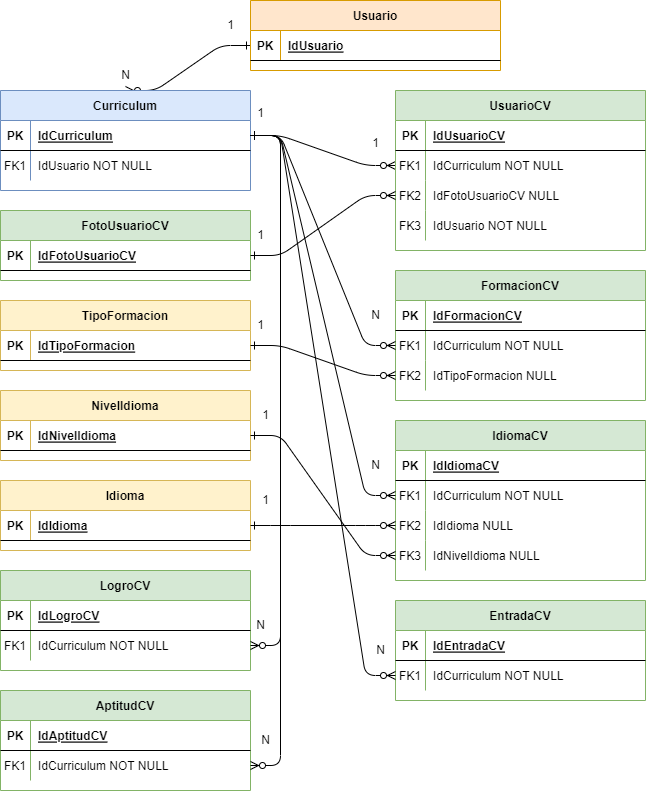
\includegraphics[width=\linewidth]{img/diagramaER_TFG.png}
    \caption{Diagrama ER - Currículos}  
\end{figure}

\begin{figure}[H]
    \centering
    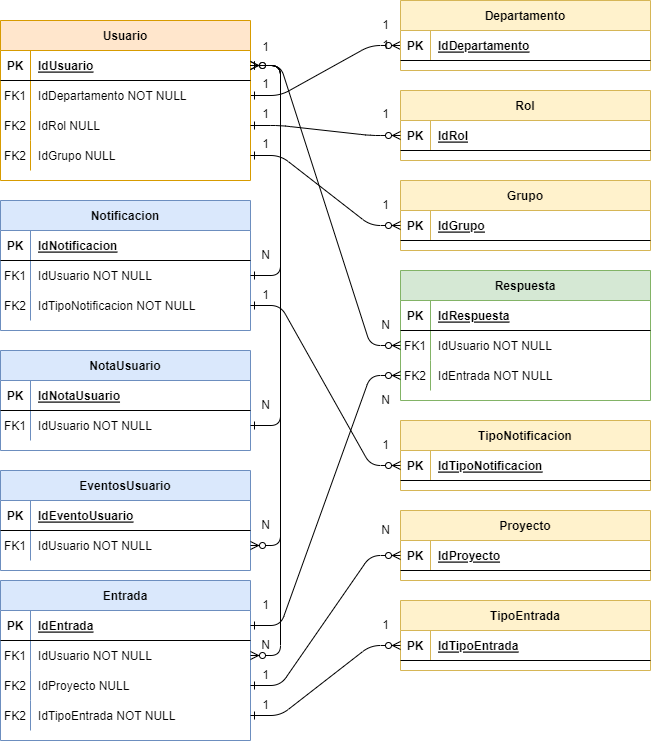
\includegraphics[width=\linewidth]{img/diagramaER2_TFG.png}
    \caption{Diagrama ER - Otros casos}  
\end{figure}

\section{Diseño estructural y funcional}
Para explicar el diseño interno de la aplicación, se va a dividir en dos categorías:
\begin{itemize}
    \item Estructura de proyectos y directorios.
    \item Instancia del programa, flujo y funcionalidad.
\end{itemize}

\subsection{Estructura interna}
La aplicación tiene los siguientes proyectos:
\begin{itemize}
    \item \textbf{Proyecto Web}: es el proyecto principal, en él se encuentra la instanciación
    de la aplicación y las configuraciones principales.
    \item \textbf{AccesoDatos}: proyecto que contiene los datos del contexto de la base de datos
    y los repositorios de los modelos para su actualización.
    \item \textbf{Modelos}: proyecto que contiene los modelos o clases referentes a la base
    de datos.
    \item \textbf{Exceptions}: proyecto del middleware de manejo de excepciones.
    \item \textbf{Logs}: en este directorio se guardan los logs de la aplicación.
    \item \textbf{Utilidades}: proyecto extra con clases comunes y/o globales.
\end{itemize}

\subsubsection{Proyecto web}
Como se ha explicado antes, es el proyecto principal. Por un lado, tiene los siguientes elementos:
\begin{itemize}
\tightlist
    \item Contiene el archivo principal de carga de la aplicación que es ``program.cs''.
    \item Tiene las configuraciones de la cadena de conexión en un ``appsettings.json''.
    \item Propiedades del lanzamiento de la aplicación (variables de entorno, puertos, etc.).
\end{itemize}

Además, posee los siguientes directorios:
\begin{itemize}
    \item \textbf{wwwroot}: carpeta root de la aplicación que contiene las hojas de estilos, scripts
    y otras carpetas de utilidad (imágenes, iconos y librerías).
    \item \textbf{Views}: carpeta contenedora de todas las vistas de la aplicación.
    \item \textbf{Controllers}: carpeta donde se guardan las clases de los controladores.
\end{itemize}

\subsubsection{AccesoDatos}
Es el proyecto que une el contexto de la base de datos con el programa, y tiene los siguientes subdirectorios:
\begin{itemize}
    \item \textbf{\emph{Data}}: contiene el archivo de instanciación del contexto y las tablas de la base de datos.
    \item \textbf{\emph{Migrations}}: guarda los cambios en la base de datos a través de migraciones y actualiza la imagen de la base de datos (este archivo contiene la estructura de la base de datos en cuanto a tablas y datos en forma de script en código de servidor).
    \item \textbf{Repositorio}: contiene las clases de los repositorios. Cada tabla tiene una
    para poder acceder a ella y cambiar u obtener datos. La instanciación depende de una interfaz
    que se realiza de la misma forma (una por cada tabla) y por último se añaden a un archivo global llamado ``UnitOfWork'', que es el medio por el que se obtienen las llamadas a dichas clases.
\end{itemize}

\subsubsection{Modelos}
Proyecto contenedor de dos partes principales del modelo:
\begin{itemize}
    \item \textbf{ViewModels}: son modelos personalizados, creados e instanciados a tiempo real
    por los controladores. Los datos se cargan como indica el programador y forman modelos cuyo
    uso principal es dotar de datos de varias tablas a una vista.
    \item \textbf{Models}: las clases de las tablas de la base de datos.
\end{itemize}

\subsection{Funcionalidad del flujo}
La funcionalidad de la aplicación sigue un flujo por pasos, a través de las dependencias entre proyectos:
\begin{itemize}
    \item 1º. Se hacen las configuraciones previas (entorno, cadena de conexión, etc).
    \item 2º. Se añaden las dependencias de los proyectos para acceder a la información de los datos de los modelos.
    \item 3º. Se configuran las librerías y los paquetes externos.
    \item 4º. Se añade el contexto de la base de datos y se añaden las vistas al lanzador.
    \item 5º. Se añaden al objeto lanzador de la aplicación las redirecciones http y la configuración básica de la web.
    \item 6º. Se indica la vista principal del lanzamiento y se ejecuta a través del entorno indicado. Si no se configuran más entornos, coge por defecto ``develop'', que es el entorno
    local.
\end{itemize}

A partir de este punto, la aplicación se ejecuta y se accede a la vista que se indica de inicio. En este momento, todo está cargado y el flujo sigue los pasos del MVC, de forma que el usuario interactúa con la vista y el controlador realizará las acciones pertinentes (redirecciones, peticiones http del tipo POST o GET, etc.).

\subsection{Dependencias y paquetes}
Todos los proyectos anteriormente mencionados tienen dependencias, no sólo entre sí, sino también a nivel de librerías. Cada proyecto guarda una relación con otro dependiendo del nivel de ejecución.

Por ejemplo, el proyecto principal depende de todos los demás, ya que es el que lanza la aplicación. Por otro lado, el proyecto de AccesoDatos solo depende de Modelos, que es al que debe llamar para obtener los datos de las tablas. Otros como Modelos, Exceptions y Utilidades, no dependen de ningún proyecto, ya que son proyectos maestros que permiten la ejecución del resto.

En cuanto a las librerías y dependencias de Microsoft y ASP.NET Core se utliza el administrador de paquetes de NuGet. NuGet es una herramienta que permite instalar versiones de dependencias que aportan funciones y librerías para su uso en determinados entornos. Por ejemplo, para poder trabajar con .NET en Core, necesitamos la dependencia del \emph{EntityFramework}, que es el que permite la instanciación del contexto de los modelos en el ámbito de Core.

Todas las librerías y dependencias de proyectos de forma interna (no entre proyectos) se administran y añaden a través de este instalador de paquetes. De la misma forma, para poder realizar migraciones con cambios a base de datos, también debemos utilizar NuGet, pero en este caso se hace a través de la consola de comandos y no a través del administrador.

\section{Diseño de las vistas y navegación}
Las vistas son la parte visual de la aplicación, y, a través de ellas, el usuario puede interactuar con el servidor. Para realizar las vistas, se ha diseñado una serie de prototipos iniciales que aporten una ligera idea de cómo se vería la aplicación

\subsection{Navegación por la web}
A continuación y para finalizar con la parte del diseño de la aplicación, se explicará cómo es la navegación por la web.
\begin{figure}[H]
    \centering
    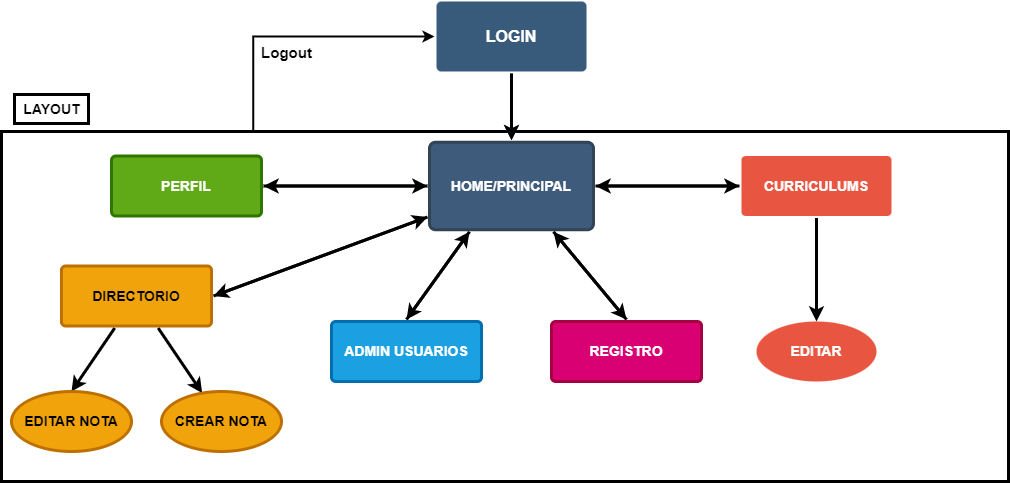
\includegraphics[width=\linewidth]{img/FlujoNavegacion.png}
    \caption{Navegación entre vistas de la aplicación}
\end{figure}


Hay varias vistas que tienen una navegación bidireccional, debido a que el layout permite:
\begin{itemize}
\tightlist
    \item Con el botón de logout volver al inicio de sesión.
    \item Volver a la página principal a través de ``Home''.
\end{itemize}

La estructura de la navegación se puede resumir en:
\begin{itemize}
\tightlist
    \item 1. \emph{Login} o inicio de sesión: vista madre de todas las demás, primera pantalla que se ve al iniciar.
    \item 2. \emph{Home}: página principal después del inicio y contenedora del layout (es el main).
    \item 3. Vistas secundarias como el perfil, los directorios, los currículums, la administración y el registro.
    \item 4. Otras vistas que se acceden a través de las anteriores, como la creación de notas y currículums, la edición de ambos, etc.
\end{itemize}


\subsection{Prototipos}
Los siguientes prototipos fueron diseñados en la fase de análisis, y forman las vistas principales de la aplicación (que no son todas, ya que muchas de las que hay en la versión final se fueron añadiendo sobre la marcha).

\begin{figure}
    \centering
    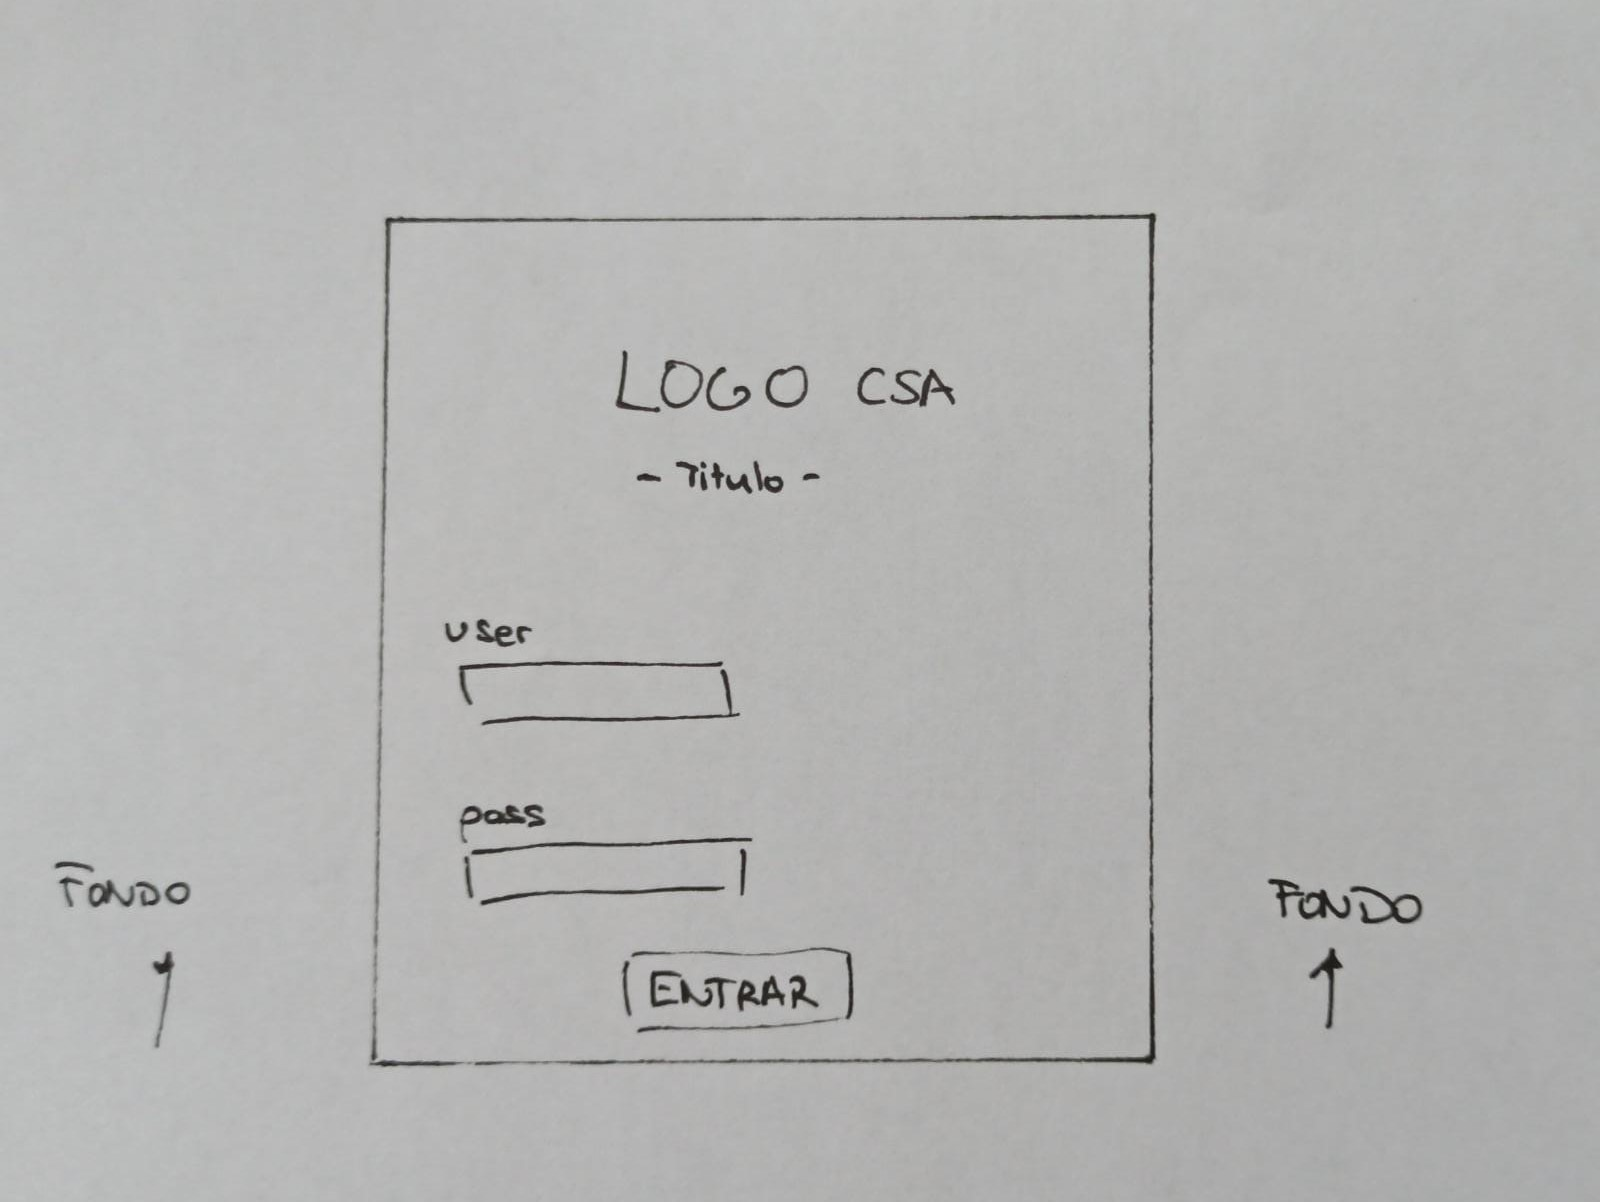
\includegraphics[width=\linewidth]{img/PT01-Login.jpeg}
    \caption{Prototipo 01. Vista del inicio de sesión}    
\end{figure}

\begin{figure}
    \centering
    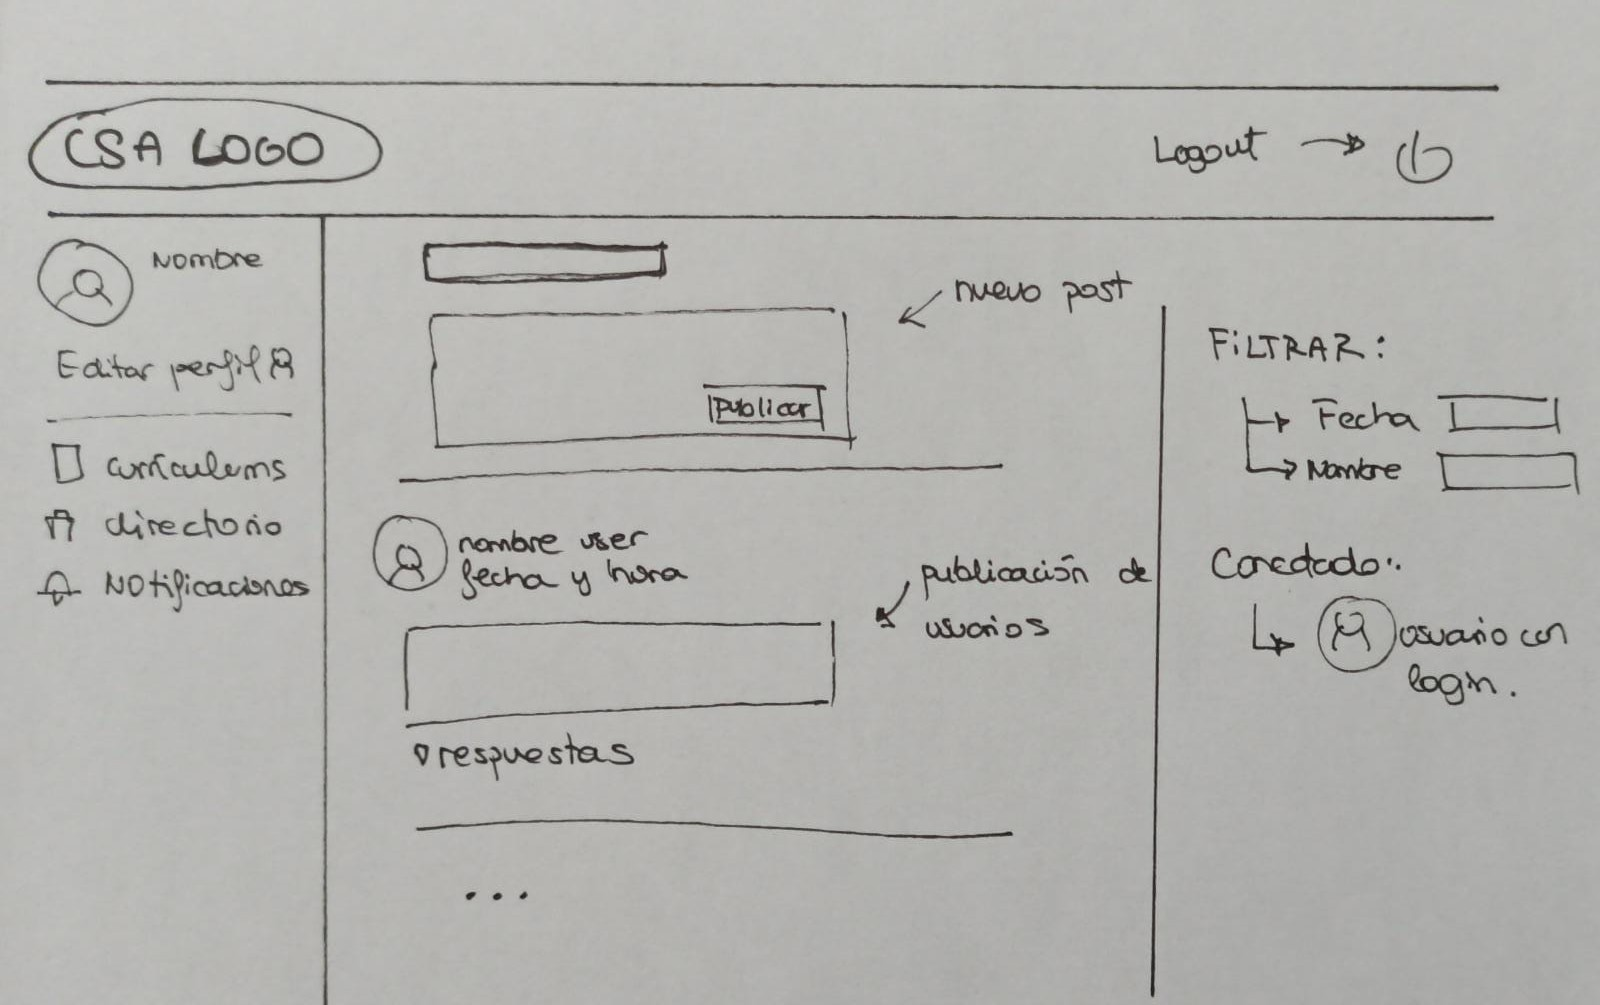
\includegraphics[width=\linewidth]{img/PT02-Home.jpeg}
    \caption{Prototipo 02. Vista principal y layout}   
\end{figure}

\begin{figure}
    \centering
    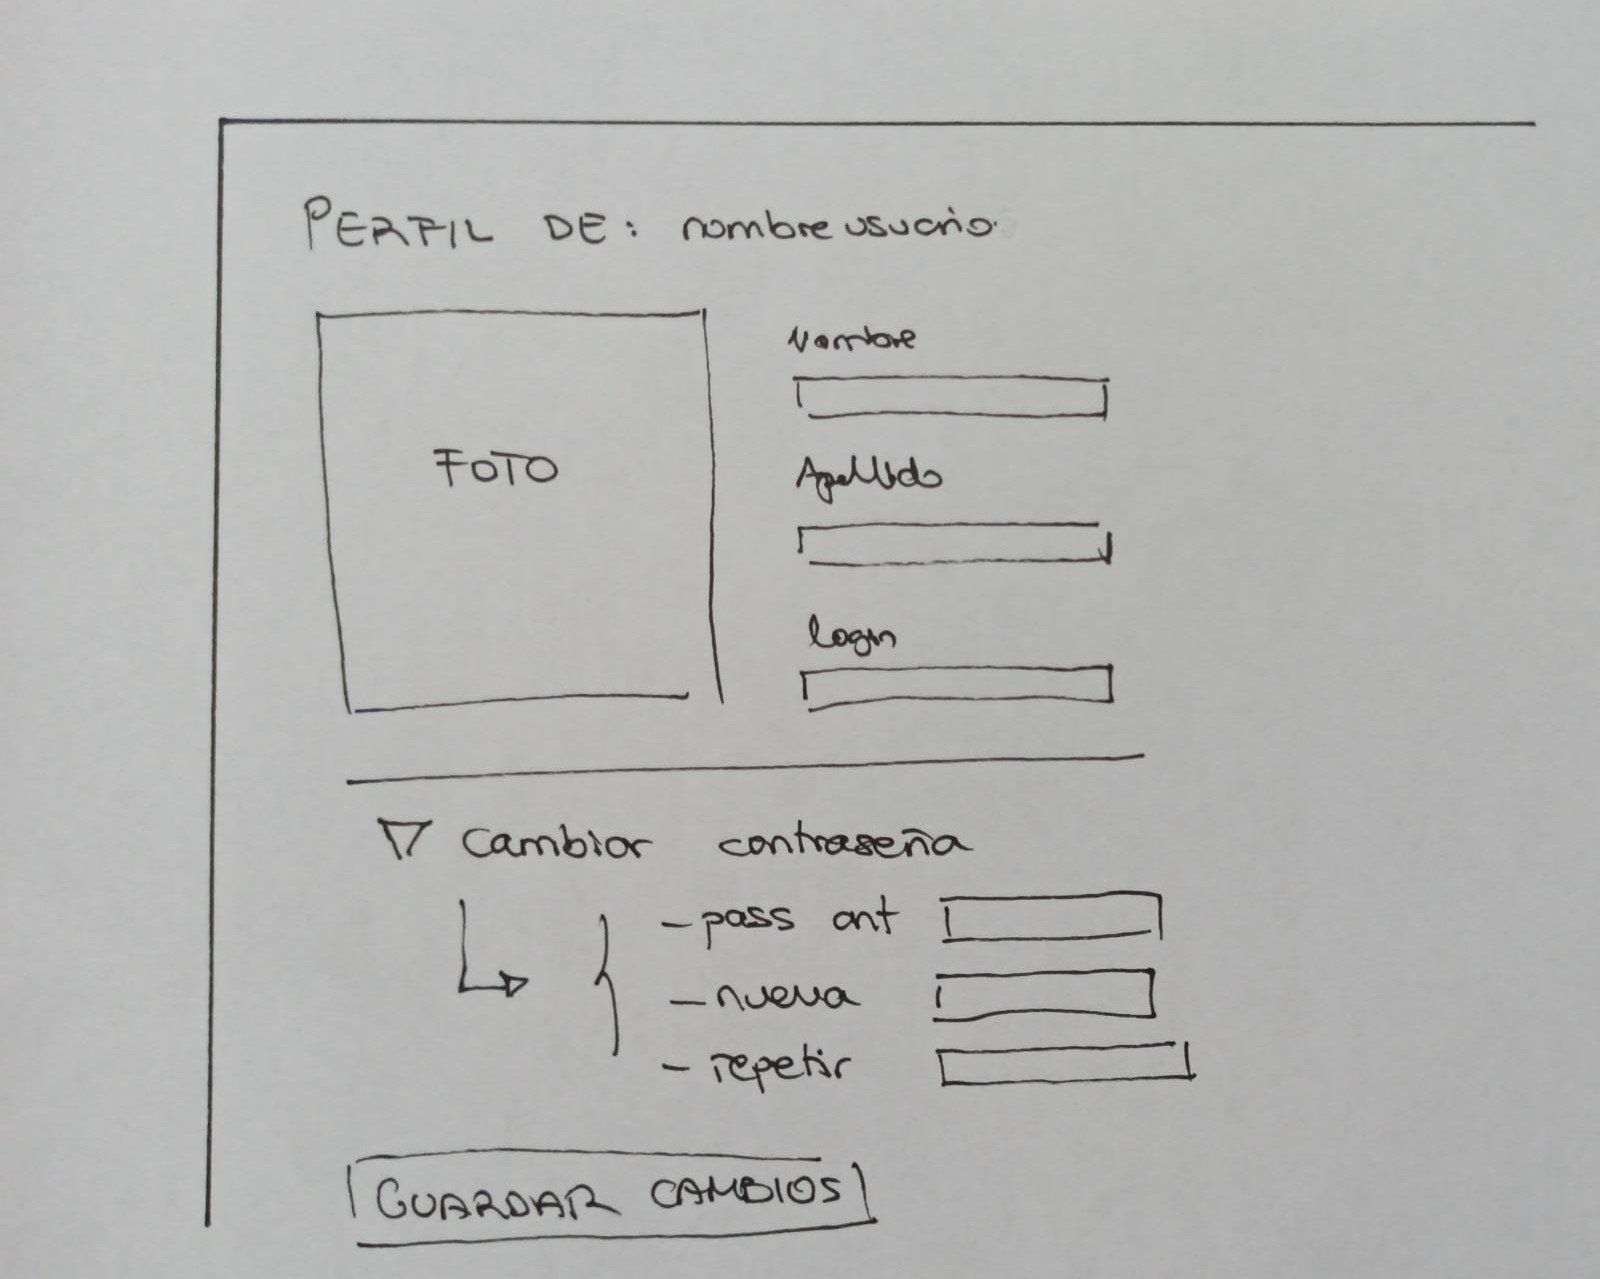
\includegraphics[width=\linewidth]{img/PT03-Profile.jpeg}
    \caption{Prototipo 03. Vista del perfil de los usuarios}    
\end{figure}

\begin{figure}
    \centering
    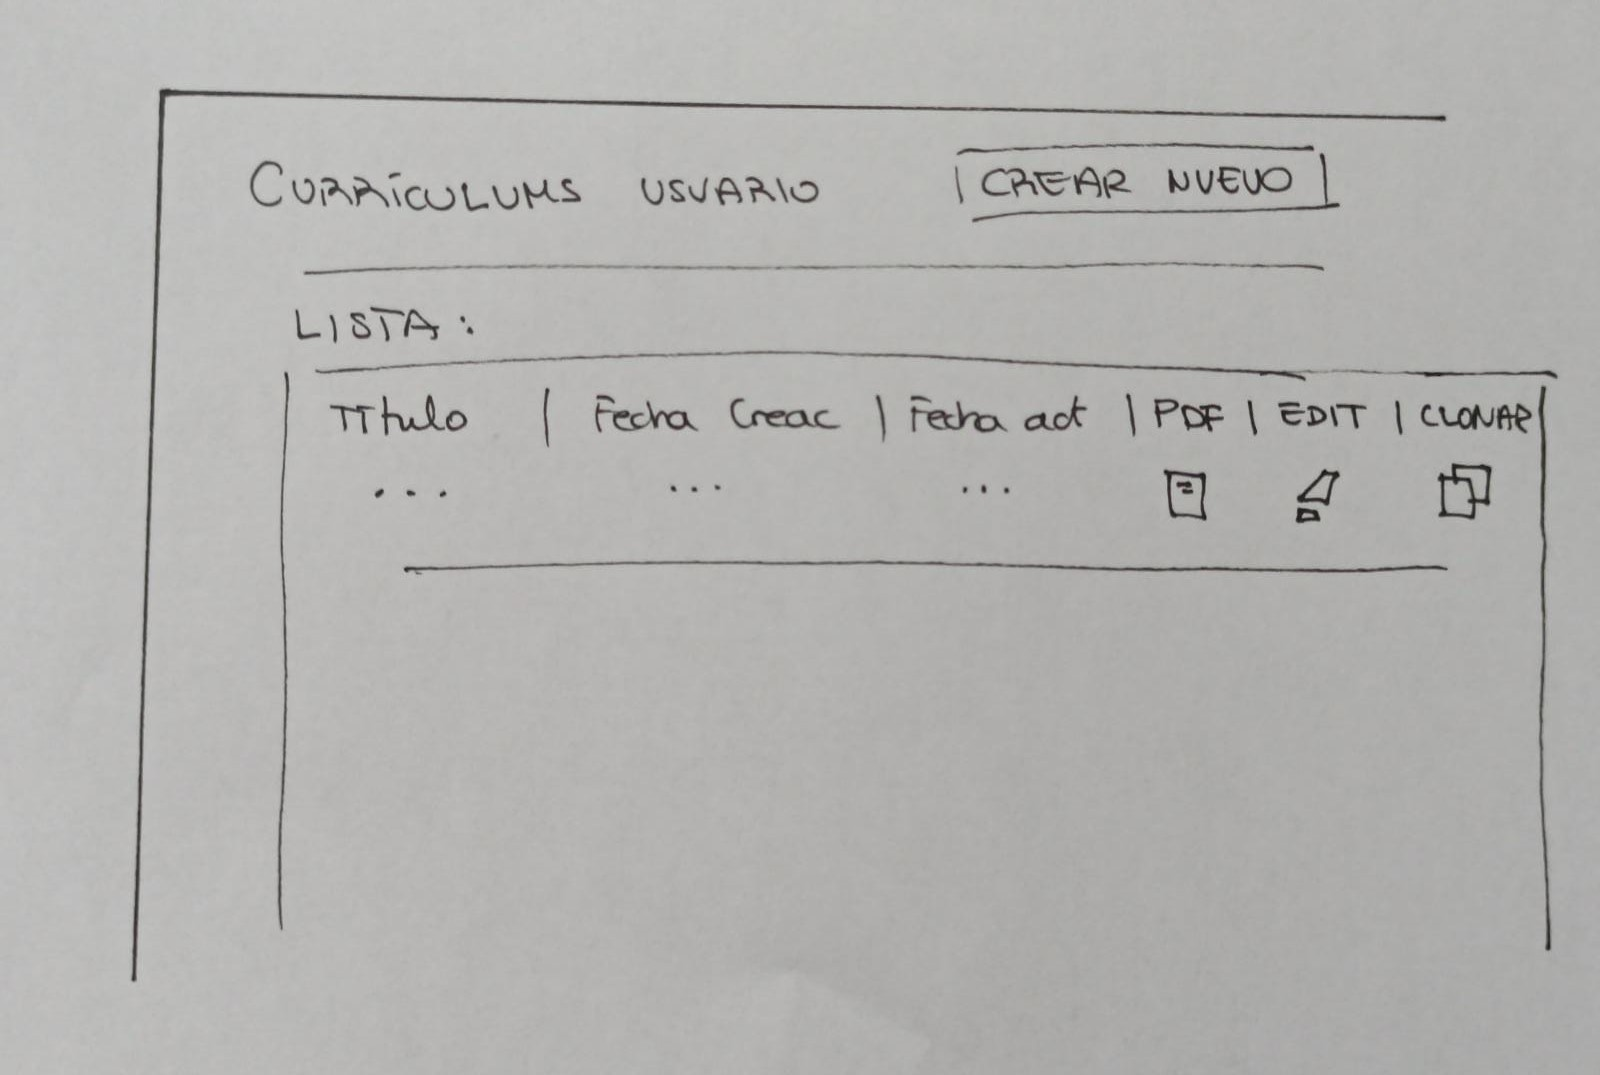
\includegraphics[width=\linewidth]{img/PT04-CVUser.jpeg}
    \caption{Prototipo 04. Vista de los currículums del usuario genérico}   
\end{figure}

\begin{figure}
    \centering
    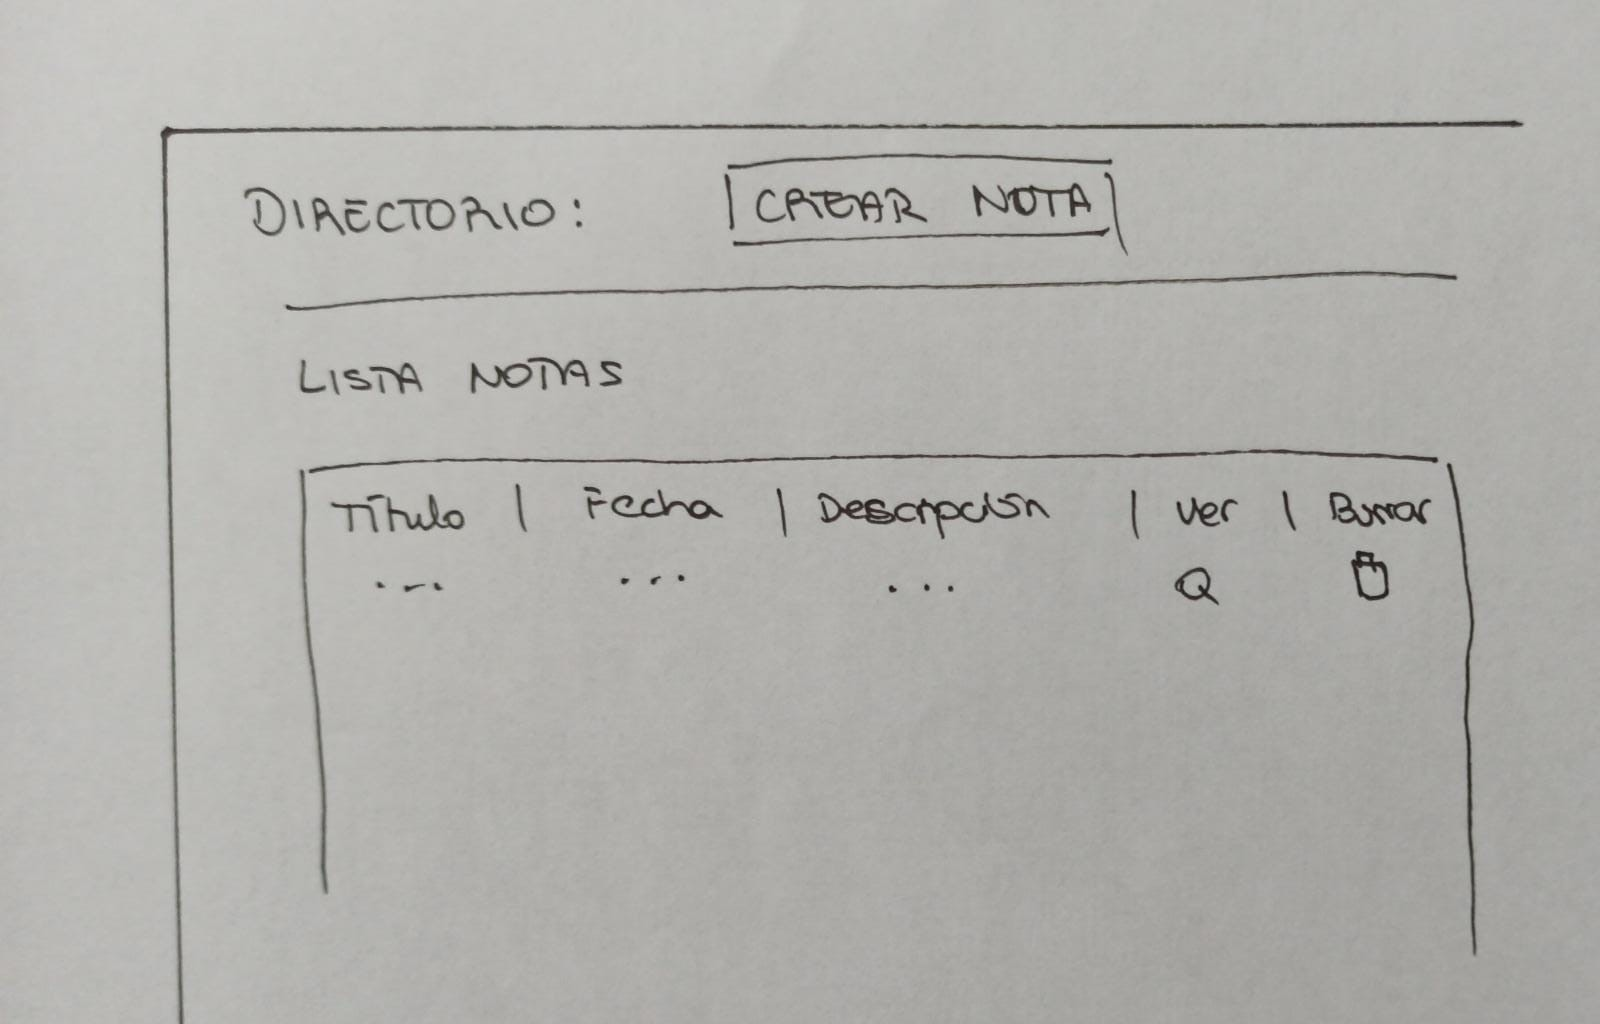
\includegraphics[width=\linewidth]{img/PT05-Directorio.jpeg}
    \caption{Prototipo 05. Vista del directorio de usuarios}
\end{figure}

\begin{figure}
    \centering
    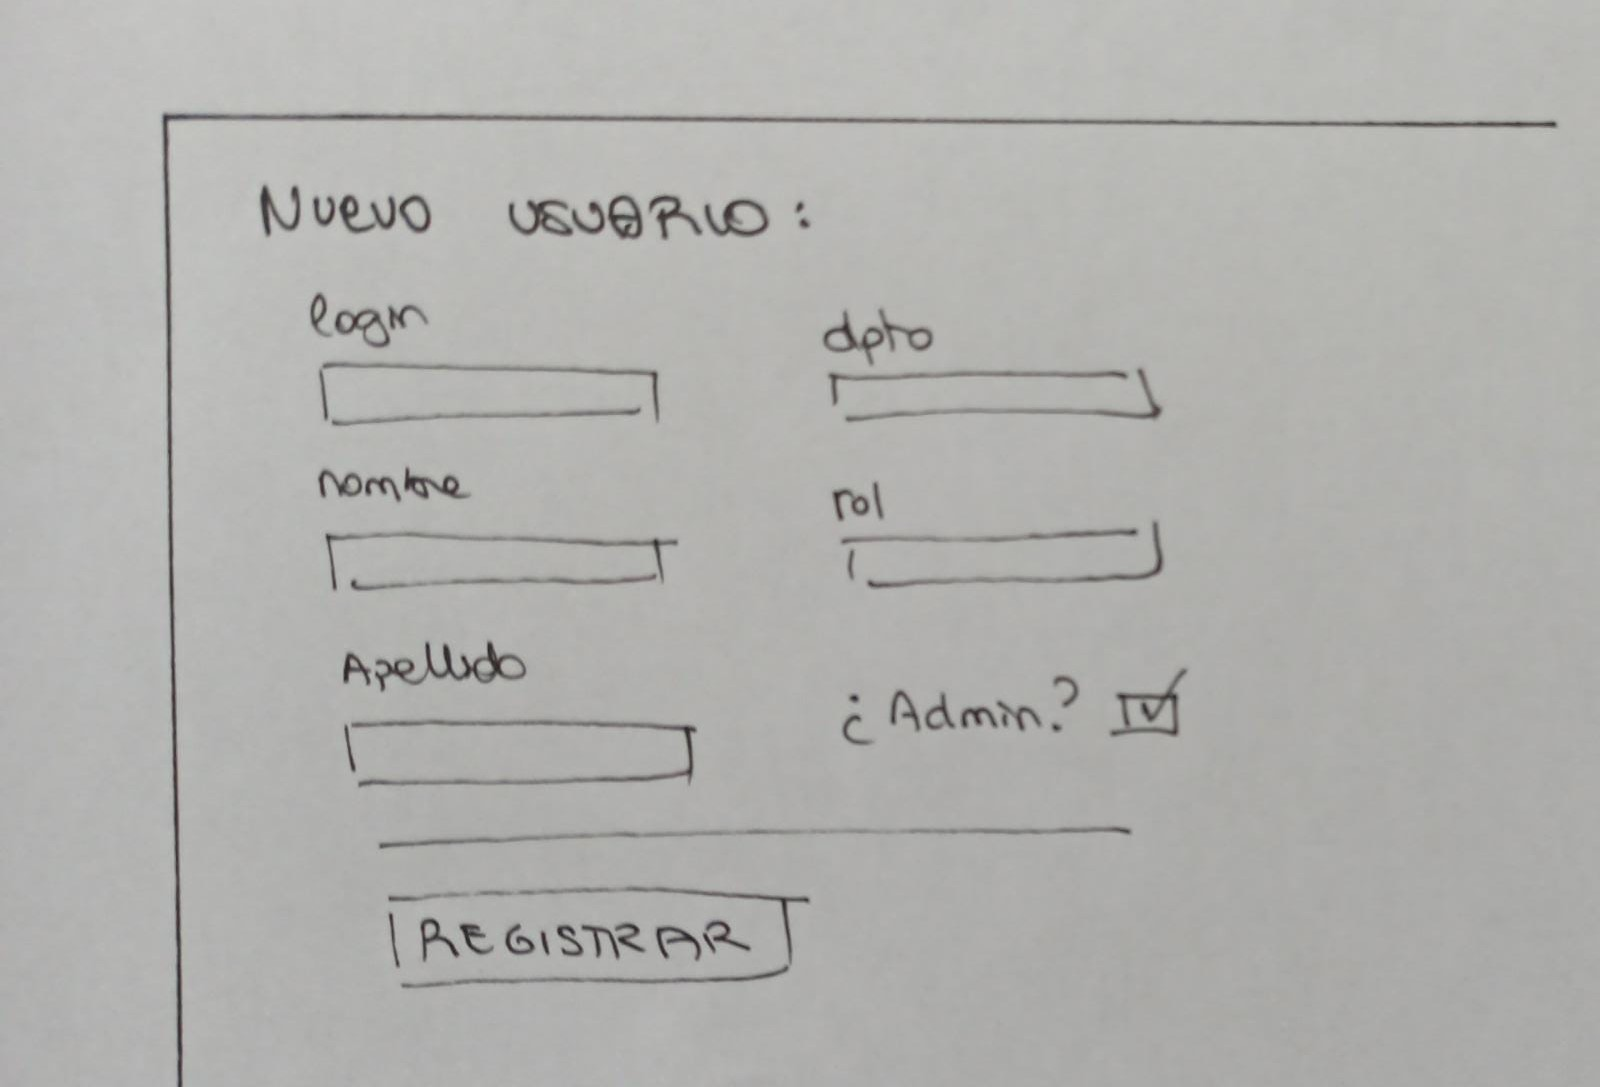
\includegraphics[width=\linewidth]{img/PT06-Register.jpeg}
    \caption{Prototipo 06. Vista del registro de usuarios}   
\end{figure}

\begin{figure}
    \centering
    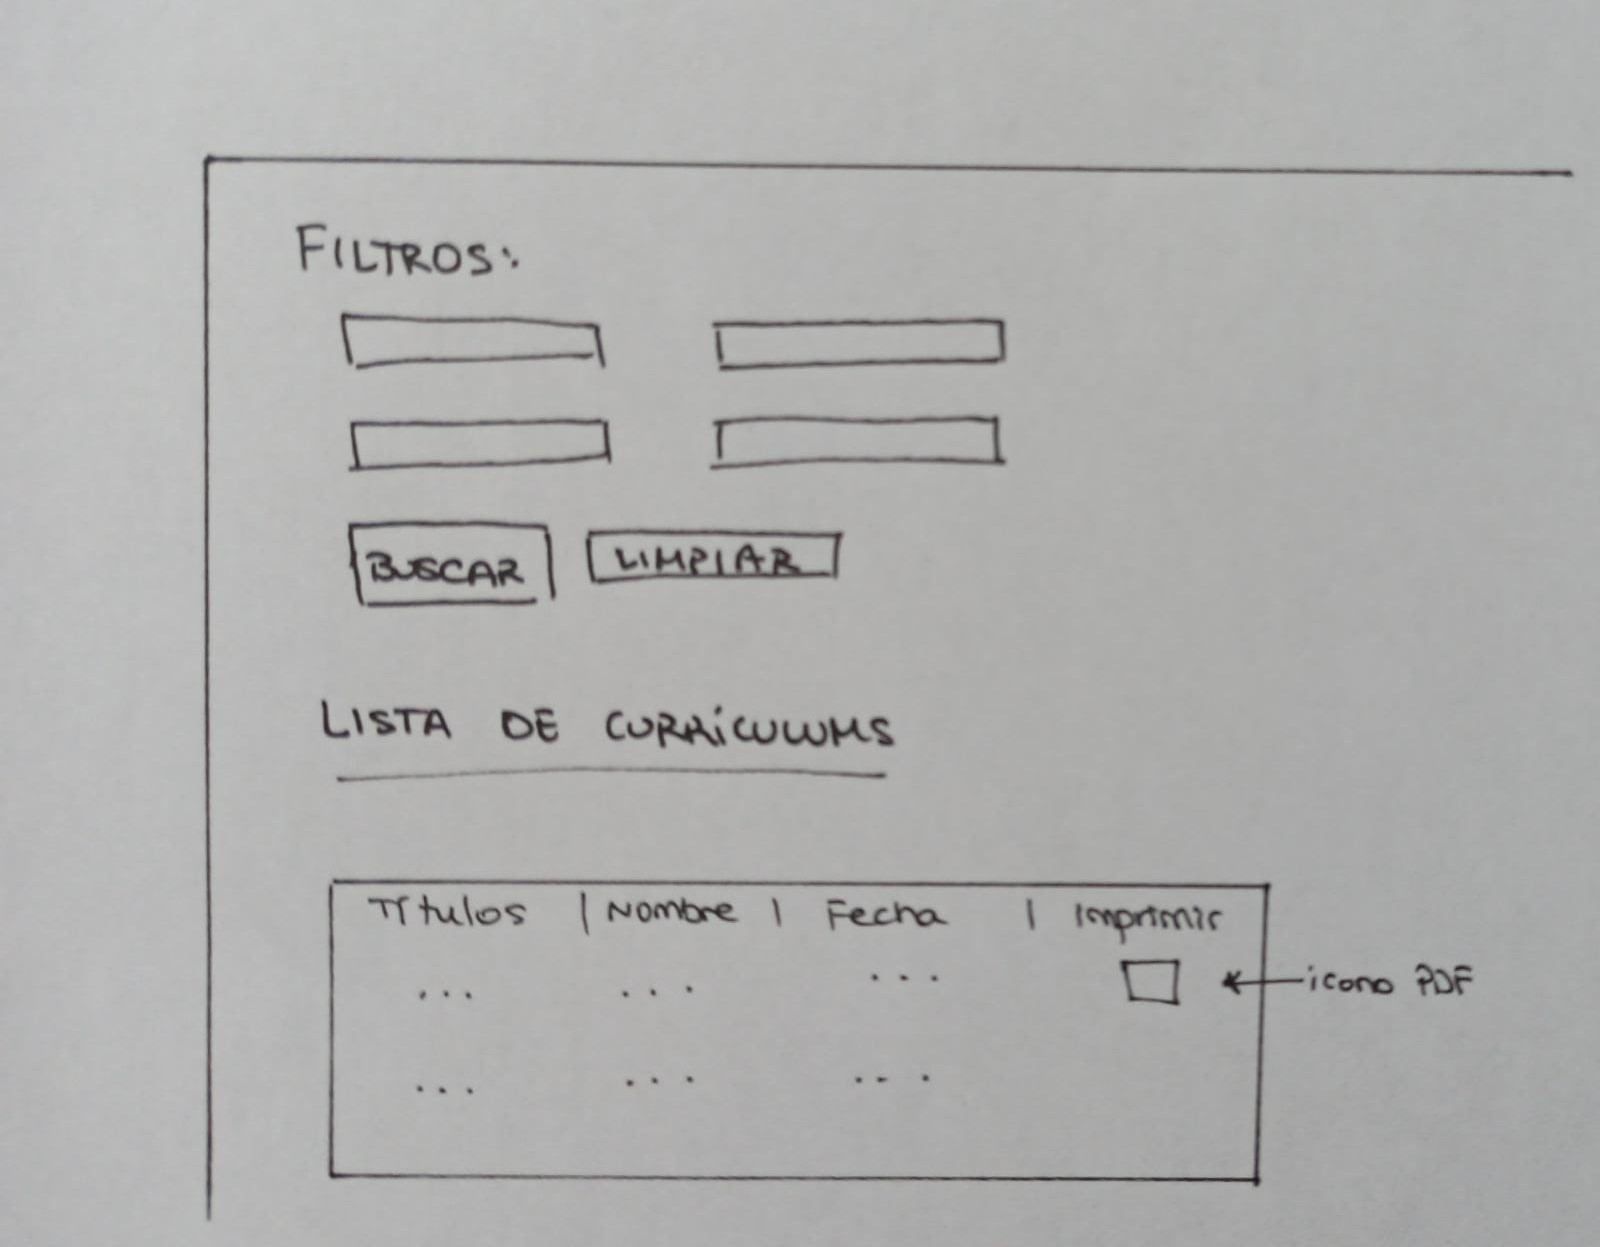
\includegraphics[width=\linewidth]{img/PT07-CVAdmin.jpeg}
    \caption{Prototipo 07. Vista de la administración de currículums}    
\end{figure}

\begin{figure}
    \centering
    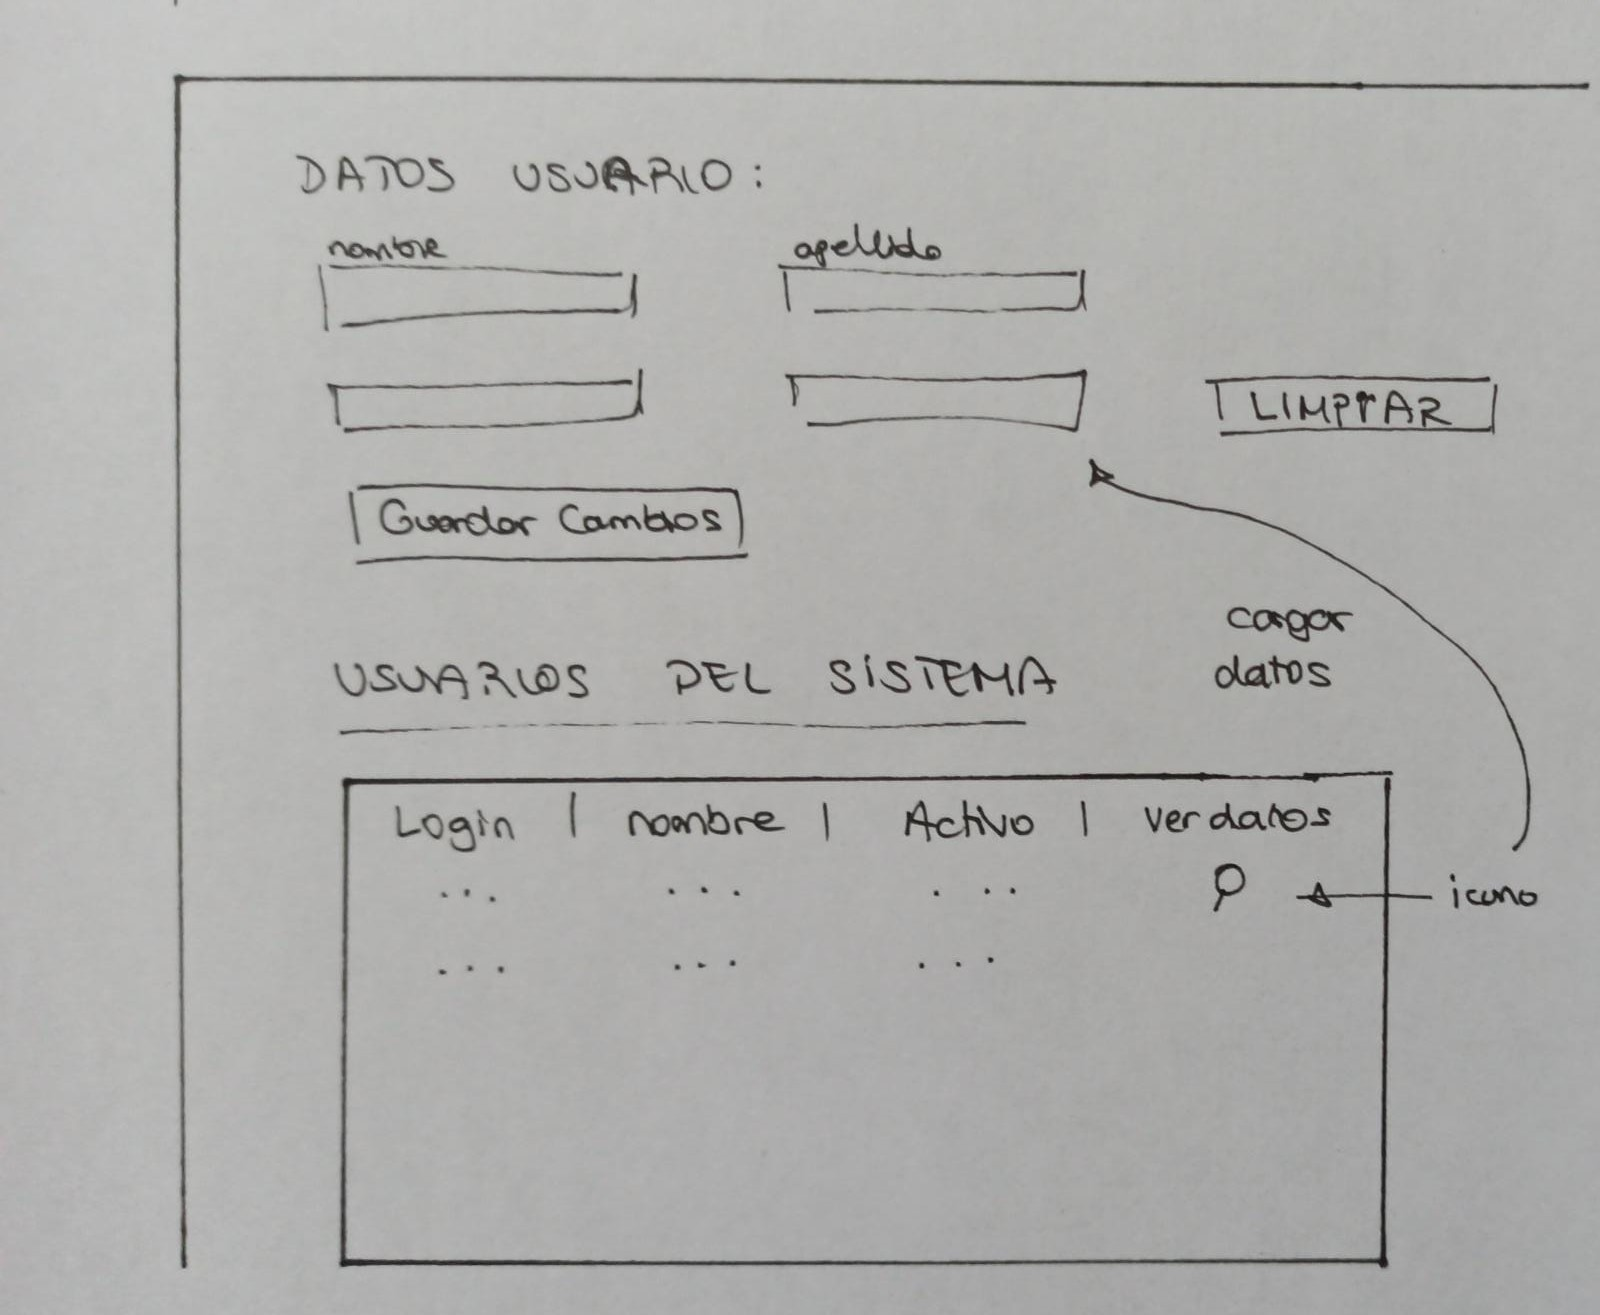
\includegraphics[width=\linewidth]{img/PT08-UserAdmin.jpeg}
    \caption{Prototipo 08. Vista de la administración de usuarios} 
\end{figure}



